\documentclass[a4paper, 12pt]{article}
\usepackage[left = 13 mm, top = 15mm, right = 13 mm, bottom = 23mm, bindingoffset = 7mm]{geometry}
\usepackage[T2A,T1]{fontenc}
\usepackage[utf8]{inputenc}
\usepackage[english,russian]{babel}
\usepackage{graphicx}
\usepackage{amssymb, mathtools}
\usepackage{lipsum}
\usepackage{float}
\usepackage{wrapfig}
\usepackage{indentfirst} 

\newcommand{\HRule}{\rule{\linewidth}{0.3mm}}

\newcommand{\LabTitle}{Эффект Холла в полупроводниках}
\begin{document}




\begin{titlepage}
\begin{center}\large
ФГАУ ВПО <<МОСКОВСКИЙ ФИЗИКО-ТЕХНИЧЕСКИЙ УНИВЕРСИТЕТ>>
\begin{figure}[H]
\centering

\includegraphics[width=15cm]{logo.jpg}
\end{figure}
{\Large
Кафедра радиотехники}

\vfill

\hrule
\vspace{0.3cm}

\huge \LabTitle

\vspace{0.3cm}
\hrule


%\noindent\rule{\textwidth}{0.4mm}
%\huge Магнитометр
%\noindent\rule{\textwidth}{0.4mm}


\end{center}

\vfill


\begin{minipage}{0.7\textwidth}
\textbf{Выполнил:}
Корепанов Г.М.

512 группа

\vspace{0.5cm}

\textbf{Преподаватель:}
Филатов Иван Васильевич
\end{minipage}


\vfill
\centering
 Долгопрудный, 2016 г.




\end{titlepage}


\section*{Теоретические выкладки}
\subsection*{Связь электрической проводимости с временем свободного пробега электрона}
{
Воспользуемся моделью свободных электронов. Между столкновениями электрон движется равноускоренно:
$$ a = \frac{eE}{m}.$$
Рассмотрим один электрон, претерпевающие много столкновений. Можно не отвлекаться на беспорядочное движение электронов, потому что оно не даёт вклада в электрический ток, то есть можно считать, что после каждого соударения электрон теряет полностью упорядоченную скорость. Тогда его средняя дрейфовая скорость найдётся из определения:
$$u = \frac{l}{\tau}=\frac{\sum a\tau_i^2/2}{\sum \tau_i}=\frac{a}{2}\frac{\overline \tau^2}{\overline \tau}.$$

Используя закон Ома $ \vec j = \lambda \vec E$ и определение плотности тока, получим выражение для электрической проводимости:
$$\lambda = \frac{ne^2}{2m}\frac{\overline \tau^2}{\overline \tau}, \text{ и}$$

\begin{equation}\label{lambda}
j= \frac{ne^2}{2m}\frac{\overline \tau^2}{\overline \tau} E_x
\end{equation}
для тока, текущего в направлении оси $Ox$.




\subsection*{Эффект Холла в модели свободных электронов}

Выведем формулы, описывающие эффект холла из классической модели свободных электронов (вообще говоря, неудовлетворительной), рассматривая ток отрицательных частиц (электронов).\footnote{Смена знака носителей никак не влияет на физическую сторону вопроса.}

Классический эффект Холла изучается только в слабых магнитных полях.\footnote{Условие слабости МП запишется в виде условия $E_y \ll E_x$, это условие соблюдается во всех элементарных экспериментах уровня лаб. работ по общей физике.} Поэтому можно пользоваться методом малых поправок (метод последовательных приближений, итерационный метод). В первом приближении внешнее МП не влияет на ток электронов по оси $Ox$:
$$\upsilon_x=\upsilon_{0x}+\frac{e}{m}E_xt.$$

Подставим это выражение в уравнение движения электронов по оси $Oy$:
$$m\dot \upsilon_y = e \left(E_y-\frac{1}{c} \upsilon_xB \right)= e\left(E_y - \frac{\upsilon_{0x}}{c}B-\frac{eB}{mc}E_x t \right).$$

Интегрируя, получим зависимость скорости от времени:
$$\upsilon_y(t) = \frac{e}{m}\left( E_y t - \frac{\upsilon_{0x}B}{c}t-\frac{eBE_x}{2m}t^2\right)$$ 

Усредним скорость электрона за время свободного пробега:
$$\overline \upsilon_y = \frac{1}{\tau}\int\limits_0^\tau \upsilon_y dt = \frac{e}{2m} \left( E_y \tau - \frac{\upsilon_{0x}B}{c} \tau - \frac{eBE_x}{2mc}\tau^2 \right).$$

Наконец, усредним по всем частицам, учитывая,  что для хаотичной системы $\overline{\upsilon_{0x}\tau} = 0$:


$$\overline \upsilon_y  = \frac{e}{2m}\left(E_y \overline{\tau} -\frac{eB}{3mc}E_x \overline{\tau^2}\right).$$

Эффект Холла соответствует установившемуся состоянию, когда сила Лоренца, действующая со стороны внешнего МП на движущиеся заряды, динамически уравновешена силой, действующей со стороны поля, созданного холловскими зарядами. Это соответствует $\overline{\upsilon_y} = 0$:
$$E_y = \frac{eB}{3mc}\frac{\overline \tau^2}{\overline \tau} E_x$$

Подставляя (\ref{lambda}), получаем результат:
\begin{equation} \label{main}
E_y=RjB,
\end{equation}
где постоянная Холла
$$R=\frac{2}{3}\frac{1}{nec}.$$


\section{Определение подвижности носителей заряда}
\section*{Расчётные формулы}
Приведём теоретическую формулу (\ref{main}) к виду, удобному для измерений. Рассмотрим пластинку длиной $L$, поперечными размерами $axl$, причем ЭДС Холла снимается с граней шириной $a$. Тогда для электронного тока
\begin{equation}\label{eds}
\varepsilon = E_yl = RjBl = -\frac{RBIl}{al}=-\frac{RBI}{a}
\end{equation}
В системе СИ формула имеет точно такой же вид, но постоянная Холла равна
$$R = \frac{1}{ne}$$
(числовой коэффициент $2/3$ опущен ввиду оценочности вывода (\ref{main})).

\section*{Экспериментальная установка}

\begin{figure}[H]
\centering
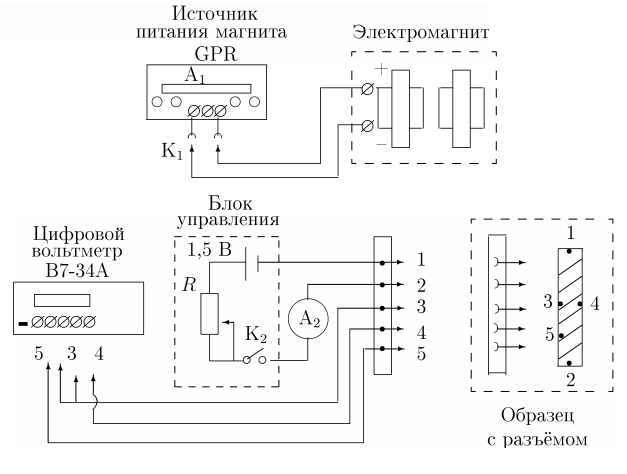
\includegraphics[scale=0.5]{1}
\caption{3,4 -- холловское напряжение, 3,5 -- измерение удельной проводимости}
\end{figure}

\section*{Эксперимент}
\subsection*{Градуировка электромагнита ($\mathbf{B(I)}$)}
Сначала определим эмпирическую зависимость индукции МП в электромагните от тока, протекающего через него, для удобства будущих измерений.
проверим исправность приборов, сопоставив их показания (в распоряжении находятся милливеберметр, прибор магнитостатической системы, и магнетометр, действие которого, как ни странно, основано на эффекте Холла) для некоторых полей, создаваемых электромагнитом:

\begin{table}[H]
\centering
\begin{tabular}{|c|c|c|c|}
\hline 
\textbf{№} & \textbf{Ток $\mathbf{I}$, А} & \textbf{Показания милливеберметра, мТл} & \textbf{Показания магнетометра, мТл} \\ 
\hline 
1 & 0,50 & 440 & 479 \\ 
\hline 
2 & 0,90 & 790 & 781 \\ 
\hline 
\end{tabular} 
\caption{Сравнение показаний приборов}
\end{table}

Как видно из таблицы, приборы работают хорошо, и, как увидим в дальнейшем, разница их показаний меньше погрешности каждого, взятого в отдельности.

\begin{table}[H]
\centering
\begin{tabular}{|l|l|l|l|}
\hline
\textbf{$\mathbf{I}$, А} & \textbf{$\mathbf{B_\leftarrow}$, мТл} & \textbf{$\mathbf{B_\rightarrow}$, мТл} & \textbf{$\mathbf{\overline B}$, мТл} \\ \hline
0,10                     & 115                                   & 114                                    & 114,5                                \\ \hline
0,20                     & 201                                   & 188                                    & 194,5                                \\ \hline
0,30                     & 292                                   & 281                                    & 286,5                                \\ \hline
0,40                     & 388                                   & 382                                    & 385                                  \\ \hline
0,50                     & 482                                   & 478                                    & 480                                  \\ \hline
0,60                     & 570                                   & 564                                    & 567                                  \\ \hline
0,70                     & 663                                   & 645                                    & 654                                  \\ \hline
0,80                     & 747                                   & 727                                    & 737                                  \\ \hline
0,90                     & 812                                   & 799                                    & 805,5                                \\ \hline
1,00                     & 883                                   & 852                                    & 867,5                                \\ \hline
\end{tabular}
\caption{Градуировка электромагнита по показаниям магнетометра в разных положениях}
\end{table}


\begin {figure}[H]
\begin{center}
% GNUPLOT: LaTeX picture with Postscript
\begingroup
  \fontfamily{sansserif}%
  \selectfont
  \makeatletter
  \providecommand\color[2][]{%
    \GenericError{(gnuplot) \space\space\space\@spaces}{%
      Package color not loaded in conjunction with
      terminal option `colourtext'%
    }{See the gnuplot documentation for explanation.%
    }{Either use 'blacktext' in gnuplot or load the package
      color.sty in LaTeX.}%
    \renewcommand\color[2][]{}%
  }%
  \providecommand\includegraphics[2][]{%
    \GenericError{(gnuplot) \space\space\space\@spaces}{%
      Package graphicx or graphics not loaded%
    }{See the gnuplot documentation for explanation.%
    }{The gnuplot epslatex terminal needs graphicx.sty or graphics.sty.}%
    \renewcommand\includegraphics[2][]{}%
  }%
  \providecommand\rotatebox[2]{#2}%
  \@ifundefined{ifGPcolor}{%
    \newif\ifGPcolor
    \GPcolorfalse
  }{}%
  \@ifundefined{ifGPblacktext}{%
    \newif\ifGPblacktext
    \GPblacktexttrue
  }{}%
  % define a \g@addto@macro without @ in the name:
  \let\gplgaddtomacro\g@addto@macro
  % define empty templates for all commands taking text:
  \gdef\gplbacktext{}%
  \gdef\gplfronttext{}%
  \makeatother
  \ifGPblacktext
    % no textcolor at all
    \def\colorrgb#1{}%
    \def\colorgray#1{}%
  \else
    % gray or color?
    \ifGPcolor
      \def\colorrgb#1{\color[rgb]{#1}}%
      \def\colorgray#1{\color[gray]{#1}}%
      \expandafter\def\csname LTw\endcsname{\color{white}}%
      \expandafter\def\csname LTb\endcsname{\color{black}}%
      \expandafter\def\csname LTa\endcsname{\color{black}}%
      \expandafter\def\csname LT0\endcsname{\color[rgb]{1,0,0}}%
      \expandafter\def\csname LT1\endcsname{\color[rgb]{0,1,0}}%
      \expandafter\def\csname LT2\endcsname{\color[rgb]{0,0,1}}%
      \expandafter\def\csname LT3\endcsname{\color[rgb]{1,0,1}}%
      \expandafter\def\csname LT4\endcsname{\color[rgb]{0,1,1}}%
      \expandafter\def\csname LT5\endcsname{\color[rgb]{1,1,0}}%
      \expandafter\def\csname LT6\endcsname{\color[rgb]{0,0,0}}%
      \expandafter\def\csname LT7\endcsname{\color[rgb]{1,0.3,0}}%
      \expandafter\def\csname LT8\endcsname{\color[rgb]{0.5,0.5,0.5}}%
    \else
      % gray
      \def\colorrgb#1{\color{black}}%
      \def\colorgray#1{\color[gray]{#1}}%
      \expandafter\def\csname LTw\endcsname{\color{white}}%
      \expandafter\def\csname LTb\endcsname{\color{black}}%
      \expandafter\def\csname LTa\endcsname{\color{black}}%
      \expandafter\def\csname LT0\endcsname{\color{black}}%
      \expandafter\def\csname LT1\endcsname{\color{black}}%
      \expandafter\def\csname LT2\endcsname{\color{black}}%
      \expandafter\def\csname LT3\endcsname{\color{black}}%
      \expandafter\def\csname LT4\endcsname{\color{black}}%
      \expandafter\def\csname LT5\endcsname{\color{black}}%
      \expandafter\def\csname LT6\endcsname{\color{black}}%
      \expandafter\def\csname LT7\endcsname{\color{black}}%
      \expandafter\def\csname LT8\endcsname{\color{black}}%
    \fi
  \fi
    \setlength{\unitlength}{0.0500bp}%
    \ifx\gptboxheight\undefined%
      \newlength{\gptboxheight}%
      \newlength{\gptboxwidth}%
      \newsavebox{\gptboxtext}%
    \fi%
    \setlength{\fboxrule}{0.5pt}%
    \setlength{\fboxsep}{1pt}%
\begin{picture}(9354.00,6802.00)%
    \gplgaddtomacro\gplbacktext{%
      \csname LTb\endcsname%
      \put(660,1408){\makebox(0,0)[r]{\strut{}$0$}}%
      \csname LTb\endcsname%
      \put(660,1949){\makebox(0,0)[r]{\strut{}$100$}}%
      \csname LTb\endcsname%
      \put(660,2489){\makebox(0,0)[r]{\strut{}$200$}}%
      \csname LTb\endcsname%
      \put(660,3030){\makebox(0,0)[r]{\strut{}$300$}}%
      \csname LTb\endcsname%
      \put(660,3570){\makebox(0,0)[r]{\strut{}$400$}}%
      \csname LTb\endcsname%
      \put(660,4111){\makebox(0,0)[r]{\strut{}$500$}}%
      \csname LTb\endcsname%
      \put(660,4651){\makebox(0,0)[r]{\strut{}$600$}}%
      \csname LTb\endcsname%
      \put(660,5192){\makebox(0,0)[r]{\strut{}$700$}}%
      \csname LTb\endcsname%
      \put(660,5732){\makebox(0,0)[r]{\strut{}$800$}}%
      \csname LTb\endcsname%
      \put(660,6273){\makebox(0,0)[r]{\strut{}$900$}}%
      \csname LTb\endcsname%
      \put(924,968){\makebox(0,0){\strut{}$0$}}%
      \csname LTb\endcsname%
      \put(2604,968){\makebox(0,0){\strut{}$0.2$}}%
      \csname LTb\endcsname%
      \put(4285,968){\makebox(0,0){\strut{}$0.4$}}%
      \csname LTb\endcsname%
      \put(5965,968){\makebox(0,0){\strut{}$0.6$}}%
      \csname LTb\endcsname%
      \put(7646,968){\makebox(0,0){\strut{}$0.8$}}%
      \csname LTb\endcsname%
      \put(9326,968){\makebox(0,0){\strut{}$1$}}%
      \put(1764,5787){\makebox(0,0)[l]{\strut{}$K = \left(861\pm17\right)$ $\frac{\text{мТл}}{\text{А}}$}}%
    }%
    \gplgaddtomacro\gplfronttext{%
      \csname LTb\endcsname%
      \put(-9,3840){\rotatebox{-270}{\makebox(0,0){\strut{}$B$, мТл}}}%
      \put(5125,308){\makebox(0,0){\strut{}$I,$ А}}%
    }%
    \gplbacktext
    \put(0,0){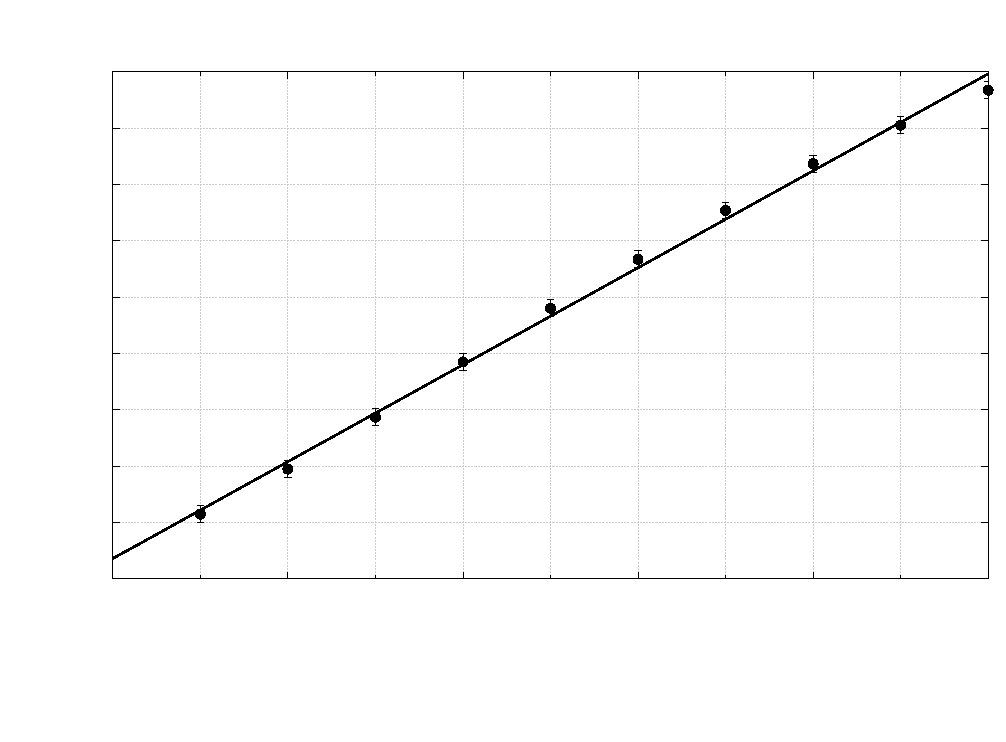
\includegraphics{plot}}%
    \gplfronttext
  \end{picture}%
\endgroup


\caption{График зависимости $B(I)$}
\end{center}

\end {figure}

В дальнейшем индукцию магнитного поля можно рассчитывать по формуле $B=KI$ с погрешностью $2\%$.

\subsection*{Параметры установки}
$$a = 1,5\text{мм}$$
$$l = 1,7\text{мм}$$
$$L_{35} = 3,0\text{мм}$$

\subsection*{Зависимость ЭДС Холла от тока через через электромагнит}
Основные экспериментальные данные, полученные в ходе эксперимента, отражены в следующих таблицах:

\begin{table}[H]
\centering
\begin{tabular}{|l|l|l|l|l|l|}
\hline
\textbf{Напряжение $U_{34}$} & \textbf{0,10 А} & \textbf{0,20 А} & \textbf{0,30 А} & \textbf{0,40 А} & \textbf{0,50 А} \\ \hline
$U_{34-1}$, мкВ              & -1              & 10              & 20              & 32              & 43              \\ \hline
$U_{34-2}$, мкВ              & 0               & 17              & 34              & 49              & 66              \\ \hline
$U_{34-3}$, мкВ              & 1               & 22              & 43              & 67              & 88              \\ \hline
$U_{34-4}$, мкВ              & 3               & 31              & 57              & 87              & 112             \\ \hline
$U_{34-5}$, мкВ              & 5               & 37              & 71              & 103             & 133             \\ \hline
$U_{34-6}$, мкВ              & 6               & 46              & 81              & 120             & 156             \\ \hline
$U_{34-7}$, мкВ              & -77             & -119            & -155            & -192            & -230            \\ \hline
\textbf{Напряжение $U_{34}$} & \textbf{0,60 А} & \textbf{0,70 А} & \textbf{0,80 А} & \textbf{0,90 А} & \textbf{1,00 А} \\ \hline
$U_{34-1}$, мкВ              & 54              & 65              & 74              & 85              & 92              \\ \hline
$U_{34-2}$, мкВ              & 83              & 97              & 112             & 125             & 138             \\ \hline
$U_{34-3}$, мкВ              & 109             & 132             & 150             & 167             & 186             \\ \hline
$U_{34-4}$, мкВ              & 138             & 164             & 188             & 210             & 228             \\ \hline
$U_{34-5}$, мкВ              & 165             & 195             & 225             & 251             & 274             \\ \hline
$U_{34-6}$, мкВ              & 193             & 226             & 261             & 292             & 322             \\ \hline
$U_{34-7}$, мкВ              & -267            & -303            & -336            & -369            & -395            \\ \hline
\end{tabular}
\caption{ЭДС Холла (исходные данные)}
\label{my-label}
\end{table}




\begin{table}[H]
\centering

\label{my-label}
\begin{tabular}{|l|l|l|l|l|l|}
\hline
\textbf{Напряжение $U_{34}$} & \textbf{0,60 А} & \textbf{0,70 А} & \textbf{0,80 А} & \textbf{0,90 А} & \textbf{1,00 А} \\ \hline
$U_{34-1}-U_0$, мкВ          & 11              & 22              & 32              & 44              & 55              \\ \hline
$U_{34-2}-U_0$, мкВ          & 15              & 32              & 49              & 64              & 81              \\ \hline
$U_{34-3}-U_0$, мкВ          & 19              & 40              & 61              & 85              & 106             \\ \hline
$U_{34-4}-U_0$, мкВ          & 24              & 52              & 78              & 108             & 133             \\ \hline
$U_{34-5}-U_0$, мкВ          & 29              & 61              & 95              & 127             & 157             \\ \hline
$U_{34-6}-U_0$, мкВ          & 33              & 73              & 108             & 147             & 183             \\ \hline
$U_{34-7}-U_0$, мкВ          & -34             & -76             & -112            & -149            & -187            \\ \hline
\textbf{Напряжение $U_{34}$} & \textbf{0,60 А} & \textbf{0,70 А} & \textbf{0,80 А} & \textbf{0,90 А} & \textbf{1,00 А} \\ \hline
$U_{34-1}-U_0$, мкВ          & 66              & 77              & 86              & 97              & 104             \\ \hline
$U_{34-2}-U_0$, мкВ          & 98              & 112             & 127             & 140             & 153             \\ \hline
$U_{34-3}-U_0$, мкВ          & 127             & 150             & 168             & 185             & 204             \\ \hline
$U_{34-4}-U_0$, мкВ          & 159             & 185             & 209             & 231             & 249             \\ \hline
$U_{34-5}-U_0$, мкВ          & 189             & 219             & 249             & 275             & 298             \\ \hline
$U_{34-6}-U_0$, мкВ          & 220             & 253             & 288             & 319             & 349             \\ \hline
$U_{34-7}-U_0$, мкВ          & -224            & -260            & -293            & -326            & -352            \\ \hline
\end{tabular}
\caption{ЭДС Холла (с компенсацией $U_0$)}
\end{table}

\begin{table}[H]
\centering
\begin{tabular}{|l|l|}
\hline
\textbf{$U_0$, мкВ} & \textbf{$I_{\text{обр}}$, мА} \\ \hline
-12                 & 0,3                           \\ \hline
-15                 & 0,44                          \\ \hline
-18                 & 0,58                          \\ \hline
-21                 & 0,72                          \\ \hline
-24                 & 0,86                          \\ \hline
-27                 & 1,00                          \\ \hline
-43                 & 1,00                           \\ \hline
\end{tabular}
\caption{Значения $U_0$ при разных значениях тока}
\label{my-label}
\end{table}



\begin {figure}[H]
\begin{center}
% GNUPLOT: LaTeX picture with Postscript
\begingroup
  \fontfamily{sansserif}%
  \selectfont
  \makeatletter
  \providecommand\color[2][]{%
    \GenericError{(gnuplot) \space\space\space\@spaces}{%
      Package color not loaded in conjunction with
      terminal option `colourtext'%
    }{See the gnuplot documentation for explanation.%
    }{Either use 'blacktext' in gnuplot or load the package
      color.sty in LaTeX.}%
    \renewcommand\color[2][]{}%
  }%
  \providecommand\includegraphics[2][]{%
    \GenericError{(gnuplot) \space\space\space\@spaces}{%
      Package graphicx or graphics not loaded%
    }{See the gnuplot documentation for explanation.%
    }{The gnuplot epslatex terminal needs graphicx.sty or graphics.sty.}%
    \renewcommand\includegraphics[2][]{}%
  }%
  \providecommand\rotatebox[2]{#2}%
  \@ifundefined{ifGPcolor}{%
    \newif\ifGPcolor
    \GPcolorfalse
  }{}%
  \@ifundefined{ifGPblacktext}{%
    \newif\ifGPblacktext
    \GPblacktexttrue
  }{}%
  % define a \g@addto@macro without @ in the name:
  \let\gplgaddtomacro\g@addto@macro
  % define empty templates for all commands taking text:
  \gdef\gplbacktext{}%
  \gdef\gplfronttext{}%
  \makeatother
  \ifGPblacktext
    % no textcolor at all
    \def\colorrgb#1{}%
    \def\colorgray#1{}%
  \else
    % gray or color?
    \ifGPcolor
      \def\colorrgb#1{\color[rgb]{#1}}%
      \def\colorgray#1{\color[gray]{#1}}%
      \expandafter\def\csname LTw\endcsname{\color{white}}%
      \expandafter\def\csname LTb\endcsname{\color{black}}%
      \expandafter\def\csname LTa\endcsname{\color{black}}%
      \expandafter\def\csname LT0\endcsname{\color[rgb]{1,0,0}}%
      \expandafter\def\csname LT1\endcsname{\color[rgb]{0,1,0}}%
      \expandafter\def\csname LT2\endcsname{\color[rgb]{0,0,1}}%
      \expandafter\def\csname LT3\endcsname{\color[rgb]{1,0,1}}%
      \expandafter\def\csname LT4\endcsname{\color[rgb]{0,1,1}}%
      \expandafter\def\csname LT5\endcsname{\color[rgb]{1,1,0}}%
      \expandafter\def\csname LT6\endcsname{\color[rgb]{0,0,0}}%
      \expandafter\def\csname LT7\endcsname{\color[rgb]{1,0.3,0}}%
      \expandafter\def\csname LT8\endcsname{\color[rgb]{0.5,0.5,0.5}}%
    \else
      % gray
      \def\colorrgb#1{\color{black}}%
      \def\colorgray#1{\color[gray]{#1}}%
      \expandafter\def\csname LTw\endcsname{\color{white}}%
      \expandafter\def\csname LTb\endcsname{\color{black}}%
      \expandafter\def\csname LTa\endcsname{\color{black}}%
      \expandafter\def\csname LT0\endcsname{\color{black}}%
      \expandafter\def\csname LT1\endcsname{\color{black}}%
      \expandafter\def\csname LT2\endcsname{\color{black}}%
      \expandafter\def\csname LT3\endcsname{\color{black}}%
      \expandafter\def\csname LT4\endcsname{\color{black}}%
      \expandafter\def\csname LT5\endcsname{\color{black}}%
      \expandafter\def\csname LT6\endcsname{\color{black}}%
      \expandafter\def\csname LT7\endcsname{\color{black}}%
      \expandafter\def\csname LT8\endcsname{\color{black}}%
    \fi
  \fi
    \setlength{\unitlength}{0.0500bp}%
    \ifx\gptboxheight\undefined%
      \newlength{\gptboxheight}%
      \newlength{\gptboxwidth}%
      \newsavebox{\gptboxtext}%
    \fi%
    \setlength{\fboxrule}{0.5pt}%
    \setlength{\fboxsep}{1pt}%
\begin{picture}(9354.00,6802.00)%
    \gplgaddtomacro\gplbacktext{%
      \csname LTb\endcsname%
      \put(660,1408){\makebox(0,0)[r]{\strut{}$0$}}%
      \csname LTb\endcsname%
      \put(660,2103){\makebox(0,0)[r]{\strut{}$1$}}%
      \csname LTb\endcsname%
      \put(660,2798){\makebox(0,0)[r]{\strut{}$2$}}%
      \csname LTb\endcsname%
      \put(660,3493){\makebox(0,0)[r]{\strut{}$3$}}%
      \csname LTb\endcsname%
      \put(660,4188){\makebox(0,0)[r]{\strut{}$4$}}%
      \csname LTb\endcsname%
      \put(660,4883){\makebox(0,0)[r]{\strut{}$5$}}%
      \csname LTb\endcsname%
      \put(660,5578){\makebox(0,0)[r]{\strut{}$6$}}%
      \csname LTb\endcsname%
      \put(660,6273){\makebox(0,0)[r]{\strut{}$7$}}%
      \csname LTb\endcsname%
      \put(924,968){\makebox(0,0){\strut{}$0$}}%
      \csname LTb\endcsname%
      \put(2324,968){\makebox(0,0){\strut{}$1$}}%
      \csname LTb\endcsname%
      \put(3725,968){\makebox(0,0){\strut{}$2$}}%
      \csname LTb\endcsname%
      \put(5125,968){\makebox(0,0){\strut{}$3$}}%
      \csname LTb\endcsname%
      \put(6525,968){\makebox(0,0){\strut{}$4$}}%
      \csname LTb\endcsname%
      \put(7926,968){\makebox(0,0){\strut{}$5$}}%
      \csname LTb\endcsname%
      \put(9326,968){\makebox(0,0){\strut{}$6$}}%
    }%
    \gplgaddtomacro\gplfronttext{%
      \csname LTb\endcsname%
      \put(176,3840){\rotatebox{-270}{\makebox(0,0){\strut{}$\tg\varphi$}}}%
      \put(5125,308){\makebox(0,0){\strut{}$1/\omega R_{\sum} C$}}%
    }%
    \gplbacktext
    \put(0,0){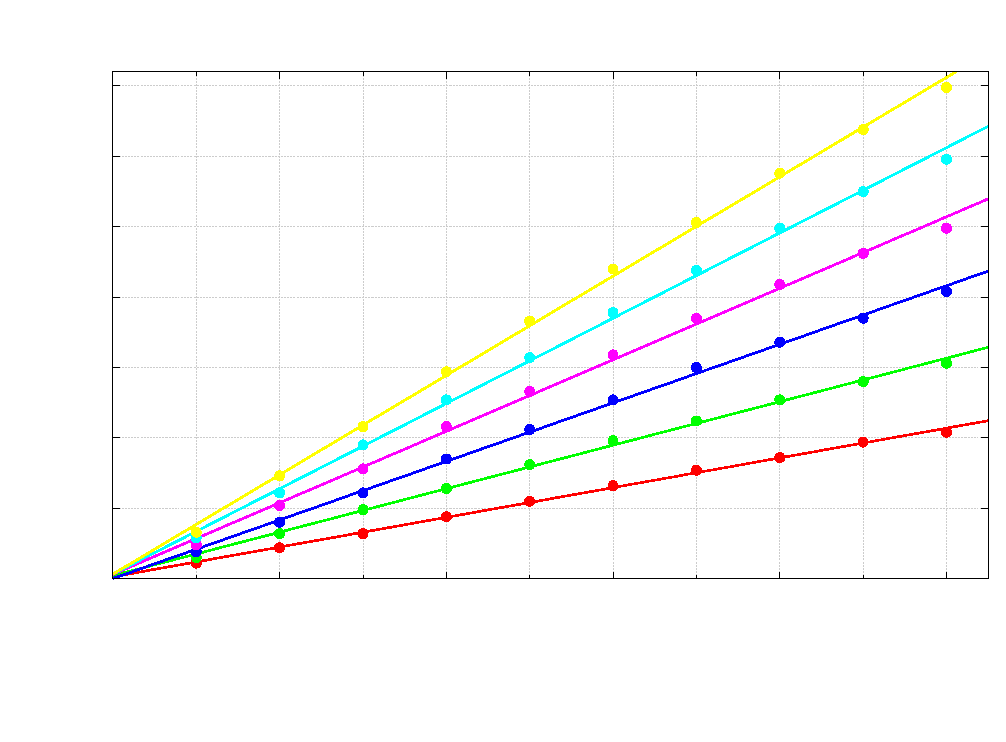
\includegraphics{plot2}}%
    \gplfronttext
  \end{picture}%
\endgroup


\caption{График зависимости $\varepsilon(I)$}
\end{center}
\end {figure}

\subsection*{Определение знака носителей}
Эффект Холла примечателен тем, что направление силы Лоренца, действующей на носители в образце, не зависит от знака носителей. Это даёт возможность по знаку ЭДС Холла определять тип проводимости:

\begin{figure}[H]
\centering
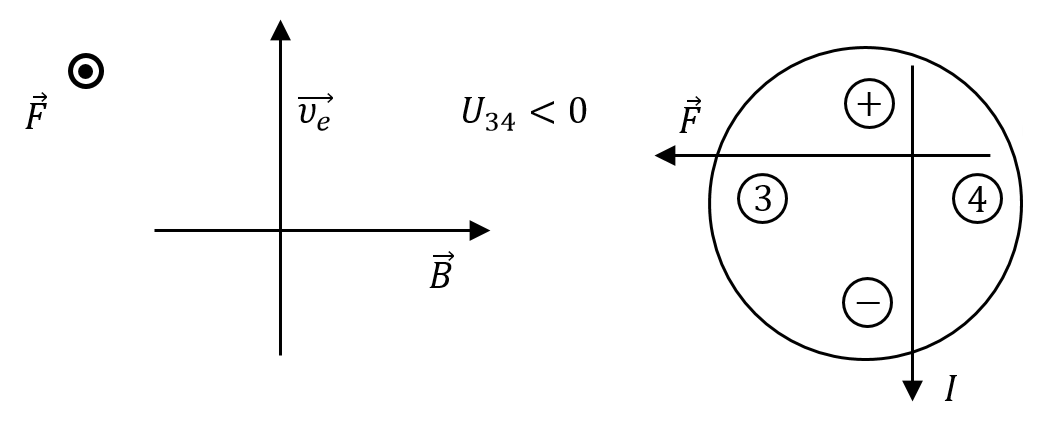
\includegraphics[width = 16cm]{sign}
\caption{Иллюстрация к определению знака носителей}
\end{figure}

Поскольку в эксперименте напряжение между контактами 3 и 4 отрицательное, то в сторону контакта 3 смещены отрицательный заряды, что говорит о преимущественной n-проводимости германия. Здесь и далее рассматриваем движение \textit{электронов}.

\subsection*{Определение постоянной Холла $\mathbf{R}$}
С хорошей точностью ЭДС Холла пропорциональная индукции магнитного поля.

В соответствии с формулой (\ref{eds}) = $\frac{RKII_\text{обр}}{a}$, откуда получаем, что коэффициенты наклона графиков $\varepsilon(I)$ равны 
$$ k_i  = \frac{RKI_\text{обр}}{a}.$$

В соответствии с этим, угловой коэффициент графика $k(I)$ даст нам при известных $a$ и $k = \frac{\Delta B}{\Delta I}$ постоянную Холла.

\begin{table}[H]
\centering
\begin{tabular}{|l|l|l|}
\hline
\textbf{$I_\text{обр}$, мА} & \textbf{$k$, $\frac{\text{мкВ}}{\text{А}}$} & \textbf{$\Delta k$, $\frac{\text{мкВ}}{\text{А}}$} \\ \hline
0,30                        & 105,58                                      & 1,59                                               \\ \hline
0,44                        & 154,48                                      & 2,46                                               \\ \hline
0,58                        & 207,94                                      & 3,08                                               \\ \hline
0,72                        & 253,94                                      & 4,72                                               \\ \hline
0,86                        & 302,85                                      & 4,77                                               \\ \hline
1,00                        & 352,79                                      & 4,66                                               \\ \hline
\end{tabular}
\caption{Зависимость коэффициента пропорциональности между ЭДС Холла и током в электромагните от тока в образце}
\label{my-label}
\end{table}

Построим график полученной зависимости:

\begin {figure}[H]
\begin{center}
% GNUPLOT: LaTeX picture with Postscript
\begingroup
  \fontfamily{sansserif}%
  \selectfont
  \makeatletter
  \providecommand\color[2][]{%
    \GenericError{(gnuplot) \space\space\space\@spaces}{%
      Package color not loaded in conjunction with
      terminal option `colourtext'%
    }{See the gnuplot documentation for explanation.%
    }{Either use 'blacktext' in gnuplot or load the package
      color.sty in LaTeX.}%
    \renewcommand\color[2][]{}%
  }%
  \providecommand\includegraphics[2][]{%
    \GenericError{(gnuplot) \space\space\space\@spaces}{%
      Package graphicx or graphics not loaded%
    }{See the gnuplot documentation for explanation.%
    }{The gnuplot epslatex terminal needs graphicx.sty or graphics.sty.}%
    \renewcommand\includegraphics[2][]{}%
  }%
  \providecommand\rotatebox[2]{#2}%
  \@ifundefined{ifGPcolor}{%
    \newif\ifGPcolor
    \GPcolorfalse
  }{}%
  \@ifundefined{ifGPblacktext}{%
    \newif\ifGPblacktext
    \GPblacktexttrue
  }{}%
  % define a \g@addto@macro without @ in the name:
  \let\gplgaddtomacro\g@addto@macro
  % define empty templates for all commands taking text:
  \gdef\gplbacktext{}%
  \gdef\gplfronttext{}%
  \makeatother
  \ifGPblacktext
    % no textcolor at all
    \def\colorrgb#1{}%
    \def\colorgray#1{}%
  \else
    % gray or color?
    \ifGPcolor
      \def\colorrgb#1{\color[rgb]{#1}}%
      \def\colorgray#1{\color[gray]{#1}}%
      \expandafter\def\csname LTw\endcsname{\color{white}}%
      \expandafter\def\csname LTb\endcsname{\color{black}}%
      \expandafter\def\csname LTa\endcsname{\color{black}}%
      \expandafter\def\csname LT0\endcsname{\color[rgb]{1,0,0}}%
      \expandafter\def\csname LT1\endcsname{\color[rgb]{0,1,0}}%
      \expandafter\def\csname LT2\endcsname{\color[rgb]{0,0,1}}%
      \expandafter\def\csname LT3\endcsname{\color[rgb]{1,0,1}}%
      \expandafter\def\csname LT4\endcsname{\color[rgb]{0,1,1}}%
      \expandafter\def\csname LT5\endcsname{\color[rgb]{1,1,0}}%
      \expandafter\def\csname LT6\endcsname{\color[rgb]{0,0,0}}%
      \expandafter\def\csname LT7\endcsname{\color[rgb]{1,0.3,0}}%
      \expandafter\def\csname LT8\endcsname{\color[rgb]{0.5,0.5,0.5}}%
    \else
      % gray
      \def\colorrgb#1{\color{black}}%
      \def\colorgray#1{\color[gray]{#1}}%
      \expandafter\def\csname LTw\endcsname{\color{white}}%
      \expandafter\def\csname LTb\endcsname{\color{black}}%
      \expandafter\def\csname LTa\endcsname{\color{black}}%
      \expandafter\def\csname LT0\endcsname{\color{black}}%
      \expandafter\def\csname LT1\endcsname{\color{black}}%
      \expandafter\def\csname LT2\endcsname{\color{black}}%
      \expandafter\def\csname LT3\endcsname{\color{black}}%
      \expandafter\def\csname LT4\endcsname{\color{black}}%
      \expandafter\def\csname LT5\endcsname{\color{black}}%
      \expandafter\def\csname LT6\endcsname{\color{black}}%
      \expandafter\def\csname LT7\endcsname{\color{black}}%
      \expandafter\def\csname LT8\endcsname{\color{black}}%
    \fi
  \fi
    \setlength{\unitlength}{0.0500bp}%
    \ifx\gptboxheight\undefined%
      \newlength{\gptboxheight}%
      \newlength{\gptboxwidth}%
      \newsavebox{\gptboxtext}%
    \fi%
    \setlength{\fboxrule}{0.5pt}%
    \setlength{\fboxsep}{1pt}%
\begin{picture}(9354.00,6802.00)%
    \gplgaddtomacro\gplbacktext{%
      \csname LTb\endcsname%
      \put(660,1408){\makebox(0,0)[r]{\strut{}$40$}}%
      \csname LTb\endcsname%
      \put(660,2016){\makebox(0,0)[r]{\strut{}$60$}}%
      \csname LTb\endcsname%
      \put(660,2624){\makebox(0,0)[r]{\strut{}$80$}}%
      \csname LTb\endcsname%
      \put(660,3232){\makebox(0,0)[r]{\strut{}$100$}}%
      \csname LTb\endcsname%
      \put(660,3841){\makebox(0,0)[r]{\strut{}$120$}}%
      \csname LTb\endcsname%
      \put(660,4449){\makebox(0,0)[r]{\strut{}$140$}}%
      \csname LTb\endcsname%
      \put(660,5057){\makebox(0,0)[r]{\strut{}$160$}}%
      \csname LTb\endcsname%
      \put(660,5665){\makebox(0,0)[r]{\strut{}$180$}}%
      \csname LTb\endcsname%
      \put(660,6273){\makebox(0,0)[r]{\strut{}$200$}}%
      \csname LTb\endcsname%
      \put(924,968){\makebox(0,0){\strut{}$0$}}%
      \csname LTb\endcsname%
      \put(2324,968){\makebox(0,0){\strut{}$50$}}%
      \csname LTb\endcsname%
      \put(3725,968){\makebox(0,0){\strut{}$100$}}%
      \csname LTb\endcsname%
      \put(5125,968){\makebox(0,0){\strut{}$150$}}%
      \csname LTb\endcsname%
      \put(6525,968){\makebox(0,0){\strut{}$200$}}%
      \csname LTb\endcsname%
      \put(7926,968){\makebox(0,0){\strut{}$250$}}%
      \csname LTb\endcsname%
      \put(9326,968){\makebox(0,0){\strut{}$300$}}%
    }%
    \gplgaddtomacro\gplfronttext{%
      \csname LTb\endcsname%
      \put(-9,3840){\rotatebox{-270}{\makebox(0,0){\strut{}$l_{max}$, мм}}}%
      \put(5125,308){\makebox(0,0){\strut{}$1/(R+R_0)$, $10^{-6} \text{ Ом}^{-1}$}}%
    }%
    \gplbacktext
    \put(0,0){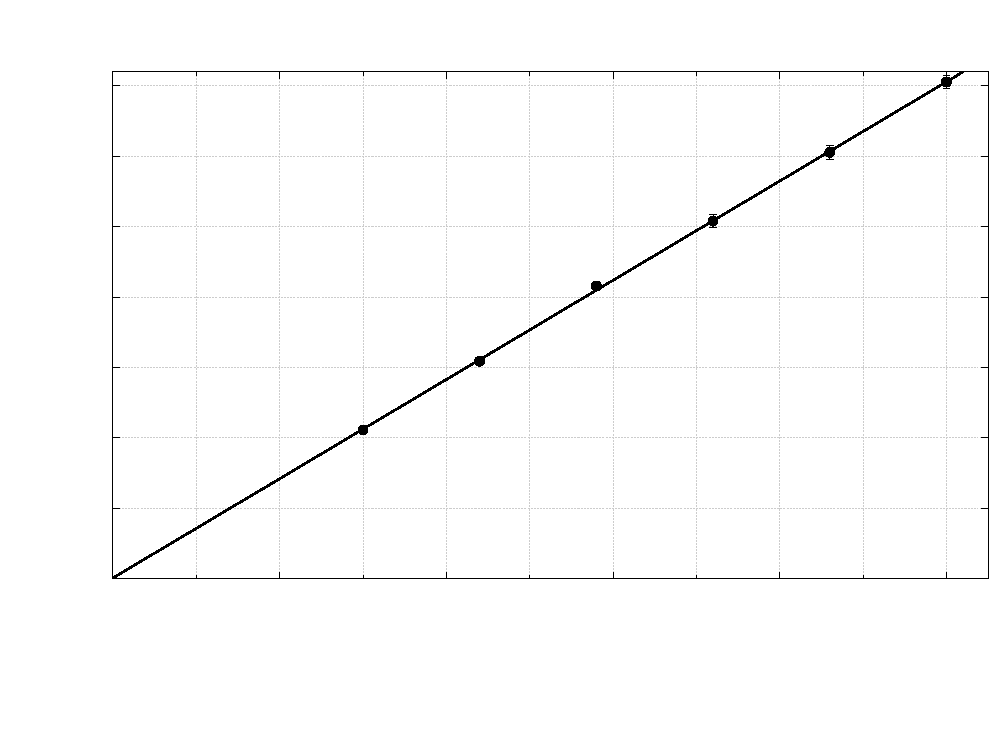
\includegraphics{plot3}}%
    \gplfronttext
  \end{picture}%
\endgroup


\caption{График зависимости $k(I)$}
\end{center}
\end {figure}

График линеен в пределах погрешностей, привычная обработка с помощью МНК даёт

$$K_1= \left(352\pm3\right)\  \frac{\text{мВ}}{\text{А}^2}=\frac{RK}{a},$$
откуда
$$R = (613\pm43)\ \frac{\text{м}^3}{\text{Кл}}$$


\section*{Определение удельной проводимости}

По определению, удельная проводимость однородного материала
$$\sigma = \frac{I_\text{обр}L_{3,5}}{U_{3,5}al}$$

Измерения дают:
\begin{table}[H]
\centering
\begin{tabular}{|l|l|}
\hline
\textbf{$U$, мВ} & \textbf{$I_\text{обр}$, мА} \\ \hline
1,716            & 1,00                        \\ \hline
1,718            & 1,00                        \\ \hline
1,715            & 1,00                        \\ \hline
\end{tabular}
\caption{Измерение проводимости}
\label{my-label}
\end{table}

$$\sigma = (685\pm54)\ \text{Ом}^{-1}\text{м}^{-1}.$$

Проводимость материала прямо зависит от подвижности электронов:

$$\sigma =enb,$$
поэтому подвижность
$$b=\frac{\sigma}{en}=\sigma R=\ (42\pm6)\frac{\text{см}^2}{\text{В}\cdot\text{с}} $$



\section*{Выводы}
\begin{itemize}
\item
Был поверхностно изучен эффект Холла на примере образца из германия.
\item
Остались без внимания вопросы, требующие использования средств квантовой механики, т.е. была изучена лишь качественная сторона вопроса. Тем не менее, как известно, формулы классической модели с точностью до числовых коэффициентов порядка 1 сходятся с результатами, полученными из квантовой механики. Поэтому выведенные законы были с хорошей точностью подтверждены экспериментом. 
\item
Изучен принцип работы милливеберметра и получен навык использования его для измерений магнитных полей.

\end{itemize}
 

\end{document}
